%%% title presenjosai2602lua
\documentclass{article}
\usepackage{geometry}
\geometry{paperwidth=148mm,paperheight=105mm}
\usepackage{luatexja}
\usepackage{pict2e}
\usepackage{ketpic2e,ketlayer2e}
\usepackage{ketslide}
\usepackage{amsmath,amssymb}
\usepackage{bm,enumerate}
\usepackage{graphicx}
\usepackage{color}
\usepackage[colorlinks=true,linkcolor=blue,filecolor=blue]{hyperref}

\usepackage{ketslide}

\usepackage{qrcode}
\usepackage{setspace}
\def\deg#1{#1^{\circ}}
\def\bs{$\backslash$}
\newcommand{\monthday}{0228}
\newcommand{\hats}{\textasciicircum}

\definecolor{slidecolora}{cmyk}{0.98,0.13,0,0.43}
\definecolor{slidecolorb}{cmyk}{0.2,0,0,0}
\definecolor{slidecolorc}{cmyk}{0.2,0,0,0}
\definecolor{slidecolord}{cmyk}{0.2,0,0,0}
\definecolor{slidecolore}{cmyk}{0,0,0,0.5}
\definecolor{slidecolorf}{cmyk}{0,0,0,0.5}
\definecolor{slidecolori}{cmyk}{0.98,0.13,0,0.43}
\def\setthin#1{\def\thin{#1}}
\setthin{0}
\newcounter{pagectr}
\setcounter{pagectr}{1}
\renewcommand{\slidepage}[1][\monthday-]{%
\setcounter{ketpicctra}{18}%

\begin{layer}{130}{0}
%\putnotew{123}{-\theketpicctra.05}{\small#1\thepage/\pageref{pageend}}
\putnotew{130}{-\theketpicctra.05}{\small#1\thepage}
\end{layer}

}

\ketslideinit

\setmargin{9}{9}{3}{3}
\pagestyle{empty}

\begin{document}

\begin{layer}{120}{0}
\putnotese{0}{0}{{\Large\bf
\color[cmyk]{1,1,0,0}

\begin{layer}{120}{0}
{\Huge \putnotes{66}{10}{和算のmnr解法における工夫}}
\putnotes{66}{21}{\huge と}
\putnotes{66}{30}{\Huge AIの利用}
\putnotes{66}{44}{髙遠 節夫}
\putnotes{66}{52}{KeTCindy センター}
\putnotes{66}{58}{日本数学教育学会名誉会員}
\putnotes{66}{66}{城西大学数学教育セミナー}
\putnotes{66}{74}{2026.02.28}
\end{layer}

}
}
\end{layer}

\def\mainslidetitley{22}
\def\ketcletter{slidecolora}
\def\ketcbox{slidecolorb}
\def\ketdbox{slidecolorc}
\def\ketcframe{slidecolord}
\def\ketcshadow{slidecolore}
\def\ketdshadow{slidecolorf}
\def\slidetitlex{6}
\def\slidetitlesize{1.3}
\def\mketcletter{slidecolori}
\def\mketcbox{yellow}
\def\mketdbox{yellow}
\def\mketcframe{yellow}
\def\mslidetitlex{62}
\def\mslidetitlesize{2}

\color{black}
\Large\bf\boldmath
\addtocounter{page}{-1}

\setthin{0.1}
\def\colorthin{\color[cmyk]{\thin,\thin,\thin,\thin}}
\setcounter{figure}{1}
%%%%%%%%%%%%

%%%%%%%%%%%%%%%%%%%%

\mainslide{和算の問題とmnr法}


\slidepage[m]
%%%%%%%%%%%%

%%%%%%%%%%%%%%%%%%%%

\newslide{mnr法とMaximaによる解法}

\vspace*{18mm}

\slidepage
\textinit[115]

\begin{layer}{120}{0}
\addtext{8}{\ten}{和算の問題を解くのは結構大変}
\addtext{8}{\ten}{和算家の卓越した計算力と知識が必要}
\addtext{16}{}{算額の問題の答と術は簡単にしか書かれていない}
\addtext{8}{\ten}{Maximaで解くことを試みた}
\addtext{16}{}{$\Rightarrow$無理式が現れて計算は破綻}
\addtext{8}{\ten}{mnr法}
\addtext{16}{}{三角形の2底角の正接$m=\tan B/2,n=\tan C/2$と内接円の半径$r$を用いる}
\addtext[6]{16}{}{$\Rightarrow$三角形の諸量は$m,n,r$の有理式となる}
\end{layer}

%%%%%%%%%%%%

%%%%%%%%%%%%%%%%%%%%


\newslide{KeTCindy}

\vspace*{18mm}

\slidepage
\textinit[120]

\begin{layer}{120}{0}
\addtext{8}{\ten}{動的幾何Cinderella2(Cindy)のライブラリ}
\addtext{8}{\ten}{TeXの描画コード(主にpict2e)ファイルを対話的に生成}
\addtext[8]{16}{}{KeTCindy$=$KeTpic$+$Cindy}
\putnotese{26}{40}{\color{blue}KeTpic$=$Kisarazu Educational Tpic(Takato)}
\addtext[8]{8}{\ten}{Maxima(,R,GCC)をKeTCindyから実行して，結果をKeTCindyで利用できる}
\addtext[8]{8}{\ten}{mnr法のためのコマンドとテンプレートを作成}
\end{layer}

%%%%%%%%%%%%

%%%%%%%%%%%%%%%%%%%%


\newslide{mnr法の主なコマンド}

\vspace*{18mm}

\slidepage
\textinit[120]

\begin{layer}{120}{0}
\addtext{2}{\ten}{\color{blue}基本コマンド}
\addtext{10}{putT(m,n,r)}{内心を原点にして三角形をおく}
\addtext{10}{slideT(p1,p2)}{p1がp2に一致するように平行移動}
\addtext{10}{rotateT(m,p)}{pの周りに(m)だけ回転}
\addtext{2}{\ten}{\color{blue}式変形の主なコマンド}
\addtext{10}{\Ltab{50mm}{numer(f),denom(f)}}{分子分母を因数分解}
\addtext{10}{\Ltab{50mm}{frfactor(f)}}{分数を簡単化}
\addtext{10}{\Ltab{50mm}{frev(eq,rep)}}{eqにrepを代入して簡単化}
\end{layer}

%%%%%%%%%%%%

%%%%%%%%%%%%%%%%%%%%


\mainslide{Malfatti円(三斜三円術)}


\slidepage[m]
%%%%%%%%%%%%

%%%%%%%%%%%%%%%%%%%%

\newslide{問題}

\vspace*{18mm}

\slidepage
\textinit[45]

\begin{layer}{120}{0}
\addtext{-2}{\ten}{安島直円}
\addtext{4}{}{不朽算法}
\addtext{10}{}{日下誠}
\addtext{10}{}{1799年}
\addtext{10}{}{写本現存}
\putnotenw{134}{76}{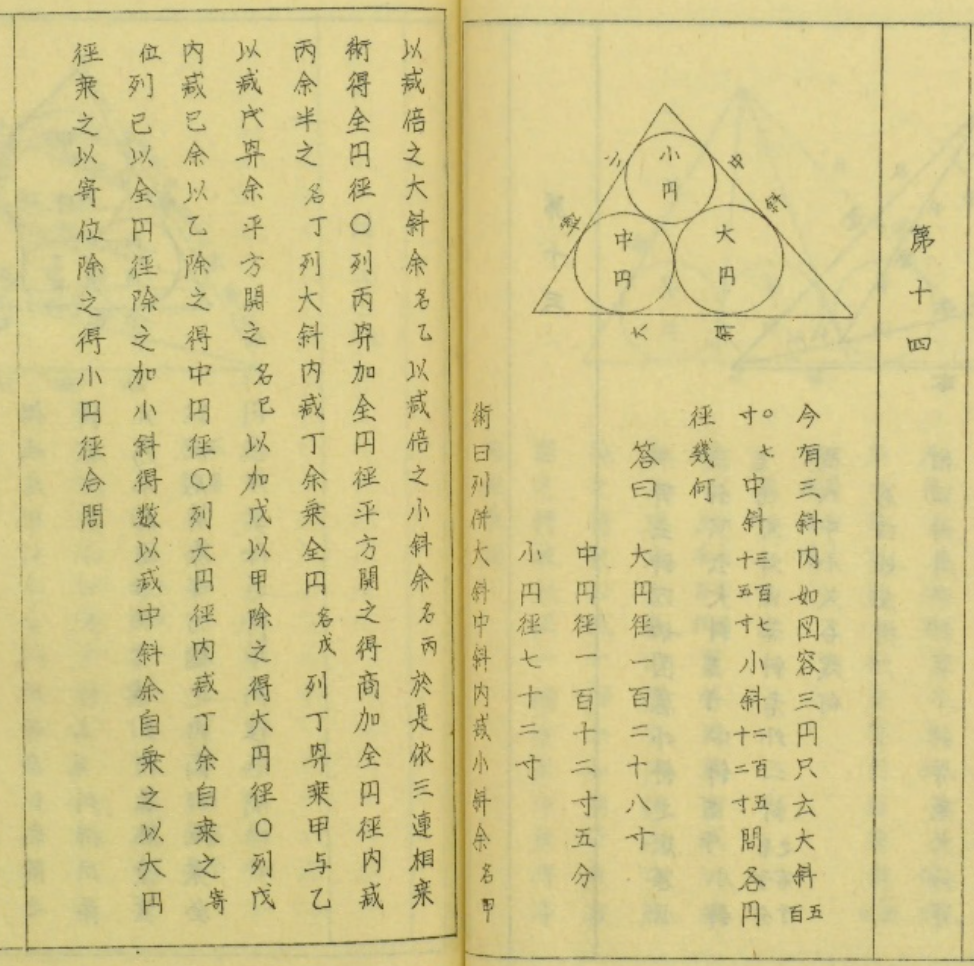
\includegraphics[height=86mm]{fig/fukyu14.png}}
\end{layer}

%%%%%%%%%%%%

%%%%%%%%%%%%%%%%%%%%


\sameslide

\vspace*{18mm}

\slidepage
\textinit[70]

\begin{layer}{120}{0}
\putnotese{80}{-12}{\scalebox{0.6}{ {\unitlength=1cm%
\begin{picture}%
(11,10)(-6,-5)%
\linethickness{0.008in}%%
\polyline(1.017,3.797)(-4.899,-2)(2.634,-2)(1.017,3.797)%
%
{%
\color[cmyk]{0,1,1,0}%
\polyline(2,0)(1.984,0.251)(1.937,0.497)(1.86,0.736)(1.753,0.964)(1.618,1.176)(1.458,1.369)%
(1.275,1.541)(1.072,1.689)(0.852,1.81)(0.618,1.902)(0.375,1.965)(0.126,1.996)(-0.126,1.996)%
(-0.375,1.965)(-0.618,1.902)(-0.852,1.81)(-1.072,1.689)(-1.275,1.541)(-1.458,1.369)%
(-1.618,1.176)(-1.753,0.964)(-1.86,0.736)(-1.937,0.497)(-1.984,0.251)(-2,0)(-1.984,-0.251)%
(-1.937,-0.497)(-1.86,-0.736)(-1.753,-0.964)(-1.618,-1.176)(-1.458,-1.369)(-1.275,-1.541)%
(-1.072,-1.689)(-0.852,-1.81)(-0.618,-1.902)(-0.375,-1.965)(-0.126,-1.996)(0.126,-1.996)%
(0.375,-1.965)(0.618,-1.902)(0.852,-1.81)(1.072,-1.689)(1.275,-1.541)(1.458,-1.369)%
(1.618,-1.176)(1.753,-0.964)(1.86,-0.736)(1.937,-0.497)(1.984,-0.251)(2,0)%
%
}%
\polyline(0.009,-0.577)(-0.002,-0.399)(-0.036,-0.223)(-0.091,-0.053)(-0.167,0.108)%
(-0.263,0.259)(-0.377,0.397)(-0.507,0.519)(-0.651,0.624)(-0.808,0.71)(-0.974,0.776)%
(-1.147,0.82)(-1.324,0.843)(-1.503,0.843)(-1.68,0.82)(-1.853,0.776)(-2.02,0.71)(-2.176,0.624)%
(-2.321,0.519)(-2.451,0.397)(-2.565,0.259)(-2.661,0.108)(-2.737,-0.053)(-2.792,-0.223)%
(-2.825,-0.399)(-2.837,-0.577)(-2.825,-0.756)(-2.792,-0.931)(-2.737,-1.101)(-2.661,-1.263)%
(-2.565,-1.413)(-2.451,-1.551)(-2.321,-1.673)(-2.176,-1.779)(-2.02,-1.865)(-1.853,-1.93)%
(-1.68,-1.975)(-1.503,-1.997)(-1.324,-1.997)(-1.147,-1.975)(-0.974,-1.93)(-0.808,-1.865)%
(-0.651,-1.779)(-0.507,-1.673)(-0.377,-1.551)(-0.263,-1.413)(-0.167,-1.263)(-0.091,-1.101)%
(-0.036,-0.931)(-0.002,-0.756)(0.009,-0.577)%
%
\polyline(2.273,-0.86)(2.264,-0.717)(2.237,-0.577)(2.193,-0.441)(2.132,-0.311)(2.055,-0.19)%
(1.964,-0.08)(1.86,0.018)(1.744,0.102)(1.618,0.171)(1.485,0.224)(1.347,0.259)(1.205,0.277)%
(1.062,0.277)(0.92,0.259)(0.781,0.224)(0.648,0.171)(0.522,0.102)(0.407,0.018)(0.302,-0.08)%
(0.211,-0.19)(0.134,-0.311)(0.073,-0.441)(0.029,-0.577)(0.002,-0.717)(-0.007,-0.86)%
(0.002,-1.003)(0.029,-1.144)(0.073,-1.28)(0.134,-1.409)(0.211,-1.53)(0.302,-1.64)%
(0.407,-1.738)(0.522,-1.823)(0.648,-1.892)(0.781,-1.944)(0.92,-1.98)(1.062,-1.998)%
(1.205,-1.998)(1.347,-1.98)(1.485,-1.944)(1.618,-1.892)(1.744,-1.823)(1.86,-1.738)%
(1.964,-1.64)(2.055,-1.53)(2.132,-1.409)(2.193,-1.28)(2.237,-1.144)(2.264,-1.003)%
(2.273,-0.86)%
%
\polyline(1.634,1.413)(1.624,1.571)(1.595,1.725)(1.546,1.875)(1.479,2.018)(1.394,2.151)%
(1.294,2.273)(1.179,2.381)(1.051,2.473)(0.913,2.549)(0.767,2.607)(0.614,2.646)(0.457,2.666)%
(0.3,2.666)(0.143,2.646)(-0.009,2.607)(-0.156,2.549)(-0.294,2.473)(-0.422,2.381)(-0.537,2.273)%
(-0.637,2.151)(-0.722,2.018)(-0.789,1.875)(-0.838,1.725)(-0.867,1.571)(-0.877,1.413)%
(-0.867,1.256)(-0.838,1.101)(-0.789,0.951)(-0.722,0.808)(-0.637,0.675)(-0.537,0.554)%
(-0.422,0.446)(-0.294,0.353)(-0.156,0.277)(-0.009,0.219)(0.143,0.18)(0.3,0.16)(0.457,0.16)%
(0.614,0.18)(0.767,0.219)(0.913,0.277)(1.051,0.353)(1.179,0.446)(1.294,0.554)(1.394,0.675)%
(1.479,0.808)(1.546,0.951)(1.595,1.101)(1.624,1.256)(1.634,1.413)%
\end{picture}%
}}}
\addtext[-4]{8}{問}{今有如三斜内容緑円及青白浅青円只浅青径若干白径若干青径若干問得緑径術如何}
\addtext[12]{24}{}{岐阜県明星輪寺算額1865}
\settext{42}{8}{105}%%
\end{layer}

%%%%%%%%%%%%

%%%%%%%%%%%%%%%%%%%%


\sameslide

\vspace*{18mm}

\slidepage
\textinit[70]

\begin{layer}{120}{0}
\putnotese{80}{-12}{\scalebox{0.6}{ {\unitlength=1cm%
\begin{picture}%
(11,10)(-6,-5)%
\linethickness{0.008in}%%
\polyline(1.017,3.797)(-4.899,-2)(2.634,-2)(1.017,3.797)%
%
{%
\color[cmyk]{0,1,1,0}%
\polyline(2,0)(1.984,0.251)(1.937,0.497)(1.86,0.736)(1.753,0.964)(1.618,1.176)(1.458,1.369)%
(1.275,1.541)(1.072,1.689)(0.852,1.81)(0.618,1.902)(0.375,1.965)(0.126,1.996)(-0.126,1.996)%
(-0.375,1.965)(-0.618,1.902)(-0.852,1.81)(-1.072,1.689)(-1.275,1.541)(-1.458,1.369)%
(-1.618,1.176)(-1.753,0.964)(-1.86,0.736)(-1.937,0.497)(-1.984,0.251)(-2,0)(-1.984,-0.251)%
(-1.937,-0.497)(-1.86,-0.736)(-1.753,-0.964)(-1.618,-1.176)(-1.458,-1.369)(-1.275,-1.541)%
(-1.072,-1.689)(-0.852,-1.81)(-0.618,-1.902)(-0.375,-1.965)(-0.126,-1.996)(0.126,-1.996)%
(0.375,-1.965)(0.618,-1.902)(0.852,-1.81)(1.072,-1.689)(1.275,-1.541)(1.458,-1.369)%
(1.618,-1.176)(1.753,-0.964)(1.86,-0.736)(1.937,-0.497)(1.984,-0.251)(2,0)%
%
}%
\polyline(0.009,-0.577)(-0.002,-0.399)(-0.036,-0.223)(-0.091,-0.053)(-0.167,0.108)%
(-0.263,0.259)(-0.377,0.397)(-0.507,0.519)(-0.651,0.624)(-0.808,0.71)(-0.974,0.776)%
(-1.147,0.82)(-1.324,0.843)(-1.503,0.843)(-1.68,0.82)(-1.853,0.776)(-2.02,0.71)(-2.176,0.624)%
(-2.321,0.519)(-2.451,0.397)(-2.565,0.259)(-2.661,0.108)(-2.737,-0.053)(-2.792,-0.223)%
(-2.825,-0.399)(-2.837,-0.577)(-2.825,-0.756)(-2.792,-0.931)(-2.737,-1.101)(-2.661,-1.263)%
(-2.565,-1.413)(-2.451,-1.551)(-2.321,-1.673)(-2.176,-1.779)(-2.02,-1.865)(-1.853,-1.93)%
(-1.68,-1.975)(-1.503,-1.997)(-1.324,-1.997)(-1.147,-1.975)(-0.974,-1.93)(-0.808,-1.865)%
(-0.651,-1.779)(-0.507,-1.673)(-0.377,-1.551)(-0.263,-1.413)(-0.167,-1.263)(-0.091,-1.101)%
(-0.036,-0.931)(-0.002,-0.756)(0.009,-0.577)%
%
\polyline(2.273,-0.86)(2.264,-0.717)(2.237,-0.577)(2.193,-0.441)(2.132,-0.311)(2.055,-0.19)%
(1.964,-0.08)(1.86,0.018)(1.744,0.102)(1.618,0.171)(1.485,0.224)(1.347,0.259)(1.205,0.277)%
(1.062,0.277)(0.92,0.259)(0.781,0.224)(0.648,0.171)(0.522,0.102)(0.407,0.018)(0.302,-0.08)%
(0.211,-0.19)(0.134,-0.311)(0.073,-0.441)(0.029,-0.577)(0.002,-0.717)(-0.007,-0.86)%
(0.002,-1.003)(0.029,-1.144)(0.073,-1.28)(0.134,-1.409)(0.211,-1.53)(0.302,-1.64)%
(0.407,-1.738)(0.522,-1.823)(0.648,-1.892)(0.781,-1.944)(0.92,-1.98)(1.062,-1.998)%
(1.205,-1.998)(1.347,-1.98)(1.485,-1.944)(1.618,-1.892)(1.744,-1.823)(1.86,-1.738)%
(1.964,-1.64)(2.055,-1.53)(2.132,-1.409)(2.193,-1.28)(2.237,-1.144)(2.264,-1.003)%
(2.273,-0.86)%
%
\polyline(1.634,1.413)(1.624,1.571)(1.595,1.725)(1.546,1.875)(1.479,2.018)(1.394,2.151)%
(1.294,2.273)(1.179,2.381)(1.051,2.473)(0.913,2.549)(0.767,2.607)(0.614,2.646)(0.457,2.666)%
(0.3,2.666)(0.143,2.646)(-0.009,2.607)(-0.156,2.549)(-0.294,2.473)(-0.422,2.381)(-0.537,2.273)%
(-0.637,2.151)(-0.722,2.018)(-0.789,1.875)(-0.838,1.725)(-0.867,1.571)(-0.877,1.413)%
(-0.867,1.256)(-0.838,1.101)(-0.789,0.951)(-0.722,0.808)(-0.637,0.675)(-0.537,0.554)%
(-0.422,0.446)(-0.294,0.353)(-0.156,0.277)(-0.009,0.219)(0.143,0.18)(0.3,0.16)(0.457,0.16)%
(0.614,0.18)(0.767,0.219)(0.913,0.277)(1.051,0.353)(1.179,0.446)(1.294,0.554)(1.394,0.675)%
(1.479,0.808)(1.546,0.951)(1.595,1.101)(1.624,1.256)(1.634,1.413)%
\end{picture}%
}}}
\addtext[-4]{8}{問}{今有如三斜内容緑円及青白浅青円只浅青径若干白径若干青径若干問得緑径術如何}
\addtext[12]{24}{}{岐阜県明星輪寺算額1865}
\settext{42}{8}{105}%%
\addtext[-8]{8}{\ten}{大村一秀の解(聖なる数学英語版 P216-218)}
\addtext{16}{}{算法点竄手引草, 1841}
\putnotese{70}{43}{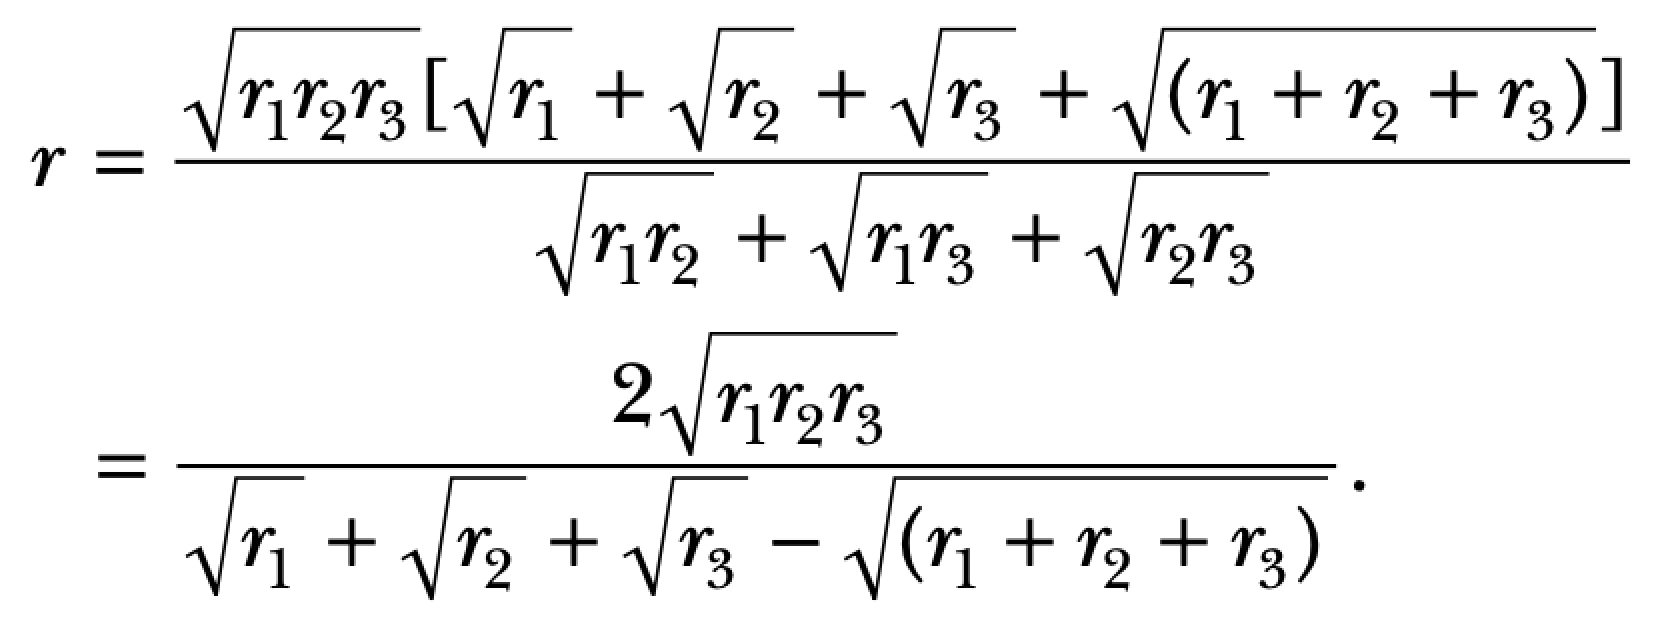
\includegraphics[height=25mm]{fig/malfattiomura.png}}
\putnotese{70}{70}{\href{https://s-takato.github.io/ketcindyorg/indexj.html}{ketcindy home}で検索}
\end{layer}

\newslide{Step1のmkcmdとcdy(Figures)}

\vspace*{18mm}

\slidepage
\textinit[115]

\begin{layer}{120}{0}
{\small
\addtext[-5]{-9}{}{mkcmd1():=(}
\addtext[-4]{-8}{}{cmdL1=concat(Mxbatch("mnr"),[}
\addtext[-4]{-8}{}{ "putT(m,n,r)",}
\addtext[-4]{-8}{}{ "A:vtxT; B:vtxL; C:vtxR; I:inC",}
\addtext[-4]{-8}{}{ "putT(m,n,s1*r); slideT(vtxL,B)",}
\addtext[-4]{-8}{}{ "D:vtxT; Eb:vtxR; I1:inC",}
\addtext[-4]{-8}{}{ "putT(m,n,s2*r); slideT(vtxR,C)",}
\addtext[-4]{-8}{}{ "G:vtxT; Ec:vtxL; I2:inC", }
\addtext[-4]{-8}{}{ "putT(m,n,s3*r); slideT(vtxT,A)",}
\addtext[-4]{-8}{}{ "H:vtxL; J:vtxR; I3:inC",}
\addtext[-4]{-8}{}{ "eq1:numer(lenSeg2(I1,I2)-(s1*r+s2*r)\hats 2)",}
\addtext[-4]{-8}{}{ "eq2:numer(lenSeg2(I2,I3)-(s2*r+s3*r)\hats 2)",}
\addtext[-4]{-8}{}{ "eq3:numer(lenSeg2(I3,I1)-(s3*r+s1*r)\hats 2)",}
\addtext[-4]{-8}{}{ "eq1:eq1/r\hats 2",}
\addtext[-4]{-8}{}{ "eq2:eq2/r\hats 2",}
\addtext[-4]{-8}{}{ "eq3:eq3/r\hats 2",}
\addtext[-4]{-8}{}{ "endstep"}
\addtext[-4]{-8}{}{ ]);}
\addtext[-4]{-8}{}{);}
%%\addtext[-14]{-7}{}{var1="A::B::C::I::D::Eb::G::Ec::H::J";}
%%\addtext[-14]{-7}{}{var1=var1+"::I1::I2::I3::eq1::eq2::eq3";}
}
\end{layer}

\textinit[115]

\begin{layer}{120}{0}
\Line(67,-10)(67,-75)
{\small
\addtext[-5]{67}{}{mkcmd1();}
\addtext[-4]{67}{}{if(contains(Ch,1),}
\addtext[-4]{67}{}{ Setmnrstep(1);}
\addtext[-4]{67}{}{ CalcbyMset(var1,"mxans1",cmdL1,op(5));}
\addtext[-4]{67}{}{ Disptex(Pos,Dy*0.75,1,var1);}
\addtext[-4]{67}{}{ s1=0.7; s2=0.6; s3=0.8;}
\addtext[-4]{67}{}{ Parsevv(var1);}
\addtext[-4]{67}{}{ dispfig1();}
\addtext[-4]{67}{}{);}
}
\end{layer}

%%%%%%%%%%%%

%%%%%%%%%%%%%%%%%%%%

\newslide{Step1を実行したcdy画面}

\vspace*{18mm}

\slidepage
\textinit[120]

\begin{layer}{120}{0}
\putnotes{65}{5}{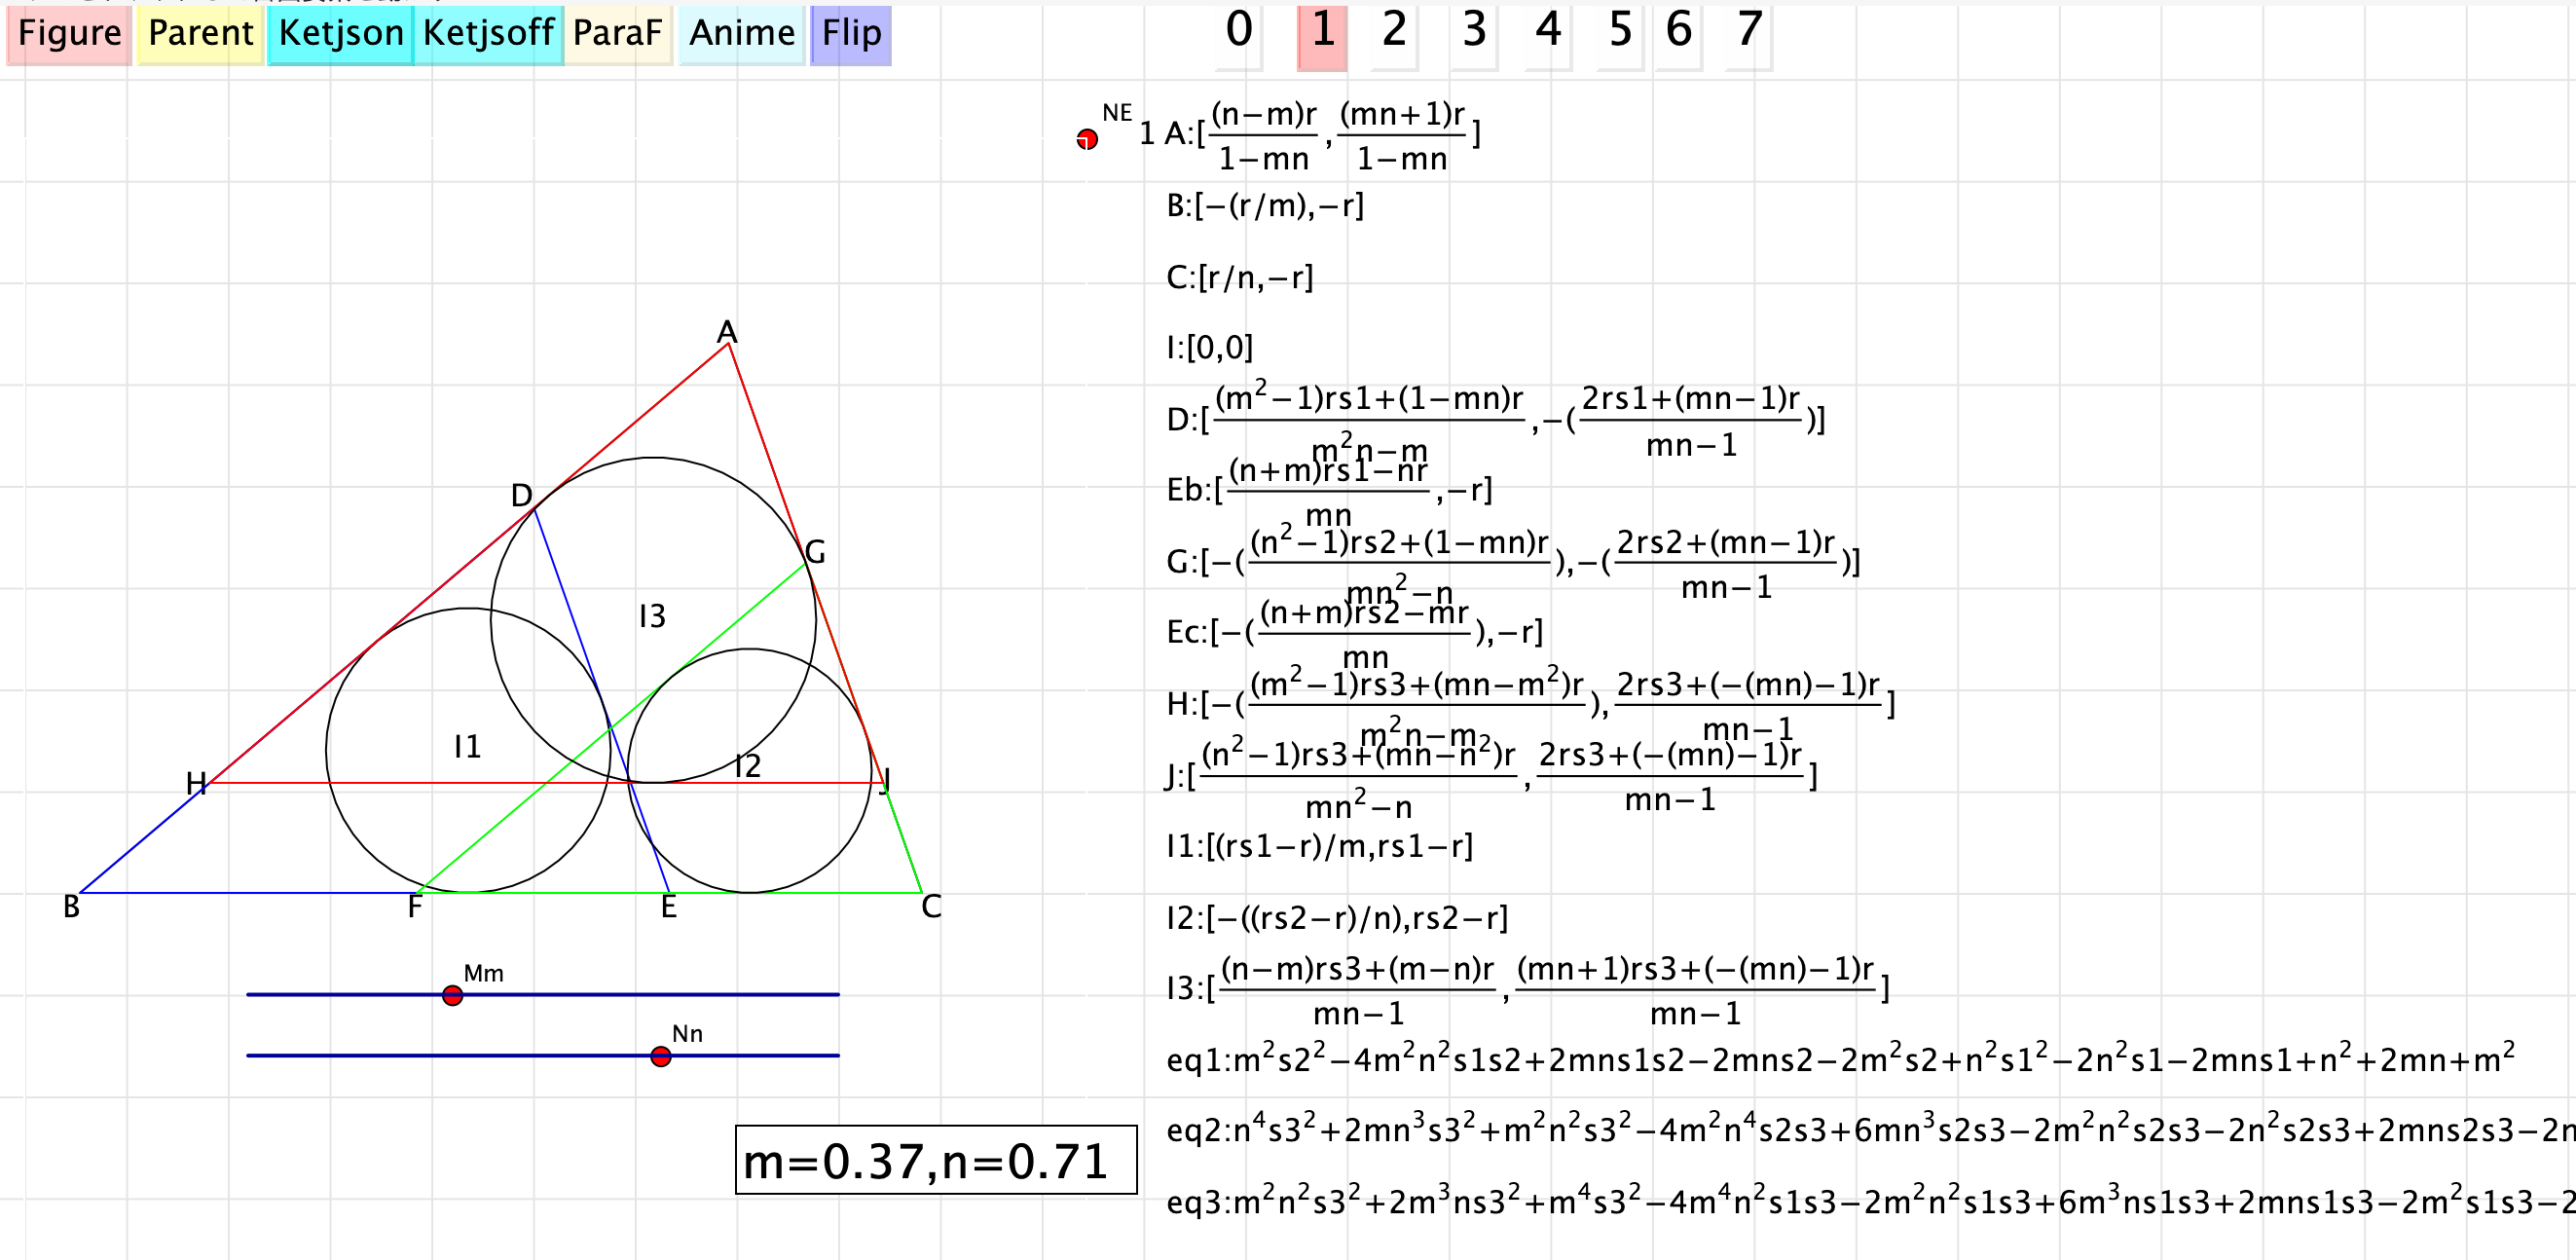
\includegraphics[width=148mm]{fig/step1sreen.png}}
\end{layer}

%%%%%%%%%%%%

%%%%%%%%%%%%%%%%%%%%

\newslide{mnr解法での工夫と着想}

\vspace*{18mm}

\slidepage
\textinit[120]

\begin{layer}{120}{0}
\addtext[-2]{8}{\ten}{最初は有理式で計算される}
\addtext{8}{\ten}{途中で4次方程式が出る}
\addtext{8}{\ten}{解は求まるが，根号の複雑な式(32個)}
\addtext{8}{\ten}{よく見ると，$\sqrt{1+m^2}$の式が出ている}
\addtext{16}{}{$\sqrt{1+m^2}=\frac{1}{\cos B/2}$}
\addtext{24}{$\Rightarrow$}{四分角の正接$M,N$の有理式}
\addtext{8}{\ten}{$M,N$に置き換えることで解を得ることができた}
\addtext{20}{}{{\color{blue}RIMS202511「数式処理の理論と応用」で発表}}
\end{layer}

%%%%%%%%%%%%

%%%%%%%%%%%%%%%%%%%%


\sameslide

\vspace*{18mm}

\slidepage
\textinit[120]

\begin{layer}{120}{0}
\addtext[-2]{8}{\ten}{最初は有理式で計算される}
\addtext{8}{\ten}{途中で4次方程式が出る}
\addtext{8}{\ten}{解は求まるが，根号の複雑な式(32個)}
\addtext{8}{\ten}{よく見ると，$\sqrt{1+m^2}$の式が出ている}
\addtext{16}{}{$\sqrt{1+m^2}=\frac{1}{\cos B/2}$}
\addtext{24}{$\Rightarrow$}{四分角の正接$M,N$の有理式}
\addtext{8}{\ten}{$M,N$に置き換えることで解を得ることができた}
\addtext{20}{}{{\color{blue}RIMS202511「数式処理の理論と応用」で発表}}
\addtext{12}{$\Rightarrow$}{最初から(または早い段階で)$M,N$を使えばどうか}
\end{layer}


\newslide{mnr解法修正版}

\vspace*{18mm}

\slidepage
\textinit[115]

\begin{layer}{120}{0}
\addtext{8}{\ten}{早い段階で$M,N$で置き換えることにする}
\end{layer}

%%%%%%%%%%%%

%%%%%%%%%%%%%%%%%%%%


\sameslide

\vspace*{18mm}

\slidepage
\textinit[115]

\begin{layer}{120}{0}
\addtext{8}{\ten}{早い段階で$M,N$で置き換えることにする}
\addtext{24}{}{{\color{blue}しかし，最初からだと式が長大になりすぎる}}
\end{layer}


\sameslide

\vspace*{18mm}

\slidepage
\textinit[115]

\begin{layer}{120}{0}
\addtext{8}{\ten}{早い段階で$M,N$で置き換えることにする}
\addtext{24}{}{{\color{blue}しかし，最初からだと式が長大になりすぎる}}
\addtext{16}{$\Rightarrow$}{式を見ながら，適切なタイミングで}
\end{layer}


\sameslide

\vspace*{18mm}

\slidepage
\textinit[115]

\begin{layer}{120}{0}
\addtext{8}{\ten}{早い段階で$M,N$で置き換えることにする}
\addtext{24}{}{{\color{blue}しかし，最初からだと式が長大になりすぎる}}
\addtext{16}{$\Rightarrow$}{式を見ながら，適切なタイミングで}
\addtext{8}{\ten}{Maximaのスクリプトが複雑になり，ミスが見つかりにくい}
\addtext[8]{16}{}{\color{red}エラーが出た時の対応に苦労する}
\end{layer}


\sameslide

\vspace*{18mm}

\slidepage
\textinit[115]

\begin{layer}{120}{0}
\addtext{8}{\ten}{早い段階で$M,N$で置き換えることにする}
\addtext{24}{}{{\color{blue}しかし，最初からだと式が長大になりすぎる}}
\addtext{16}{$\Rightarrow$}{式を見ながら，適切なタイミングで}
\addtext{8}{\ten}{Maximaのスクリプトが複雑になり，ミスが見つかりにくい}
\addtext[8]{16}{}{\color{red}エラーが出た時の対応に苦労する}
\addtext{24}{$\Rightarrow$}{Gemini Proとの対話で進めることにした}
\end{layer}


\mainslide{Geminiとの対話}


\slidepage[m]
%%%%%%%%%%%%

%%%%%%%%%%%%%%%%%%%%

\newslide{対話1 ライブラリの確認}

\vspace*{18mm}

\slidepage
\textinit[120]

\begin{layer}{120}{0}
\addtext{5}{{\color{blue}User:}}{\color{blue}和算図形問題をKeTCindyとMaximaで解きたい}
\addtext{12}{}{専用ライブラリ(\texttt{ketcindylib}, \texttt{mnr.max})の認知確認}
\addtext{12}{}{未知の場合，ファイル添付の提案}
%%\putnotese{110}{-5}{
\includegraphics[width=3cm]{fig/ai_partner.png}}
\addtext{5}{{\color{magenta}Gemini:}}{\color{magenta}協力の申し出と懸念}
\addtext{12}{}{KeTCindyやMaximaの一般的な文法は熟知}
\addtext{12}{}{特定ライブラリの内部定義は未学習の可能性大}
\addtext{12}{}{具体的な関数仕様やデータ形式の確認要望}
\addtext{16}{$\Rightarrow$}{ファイルアップロード(添付)の依頼}
\end{layer}

%%%%%%%%%%%%

%%%%%%%%%%%%%%%%%%%%


\newslide{対話2：提案された進め方}

\vspace*{18mm}

\slidepage
\textinit[120]

\begin{layer}{120}{0}
\addtext{5}{{\color{magenta}Gemini:}}{\color{magenta}ファイル受領後のサポート手順提案}
\addtext{6}{1.}{ライブラリの解析}
\addtext{10}{}{\texttt{mnr.max}等の定義読込，利用可能関数の特定}
\addtext{6}{2.}{問題の定式化}
\addtext{10}{}{和算問題をMaximaで解ける連立方程式へ定式化}
\addtext{6}{3.}{スクリプト作成}
\addtext{10}{}{図形描画(KeTCindy)と計算(Maxima)の連携コード提示}
%%\putnotese{80}{30}{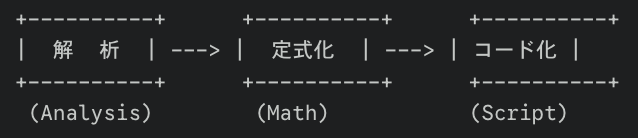
\includegraphics[width=6cm]{fig/workflow_diagram.png}}
\end{layer}

%%%%%%%%%%%%

%%%%%%%%%%%%%%%%%%%%


\newslide{最初の壁：Grobner基底}

\vspace*{18mm}

\slidepage
\textinit[120]

\begin{layer}{120}{0}
\addtext[-4]{5}{\color{blue}User:}{\color{blue}提案コードを実行したがうまくいかない}
\addtext[-1]{12}{}{\texttt{gb} (Grobner基底) が計算されず変数のまま残る}
\addtext[-1]{12}{}{リストの途中に \texttt{end} タグが含まれている}
\addtext[-1]{5}{\color{magenta}Gemini:}{\color{magenta}原因特定と方針転換}
\addtext[-1]{16}{}{1. \texttt{end}タグがMaximaの読み込みを中断させていた}
\addtext[-1]{16}{}{2. Malfattiの問題はGrobner基底では計算量爆発}
\addtext[-1]{5}{\color{magenta}Gemini:}{\color{magenta}新しいアプローチ}
\addtext[-1]{16}{}{計算コストの高いGrobner基底を諦める}
\addtext[-1]{16}{}{確実に解ける\textbf{消去法(\texttt{reduceD})}へ切り替える}
\addtext[-1]{16}{}{\texttt{end}タグを自動削除する処理を追加する}
\end{layer}

%%%%%%%%%%%%

%%%%%%%%%%%%%%%%%%%%


\newslide{消去法の調整}

\vspace*{18mm}

\slidepage
\textinit[120]

\begin{layer}{120}{0}
\addtext[-4]{5}{\color{blue}User:}{\texttt{reduceD}の試行錯誤}
\addtext{12}{}{変数が消えずに残存 ($s_2$など)}
\addtext{12}{}{中間式が長大で計算終わらず}
\addtext{5}{\color{magenta}Gemini:}{\color{magenta}パラメータの調整}
\addtext{12}{}{消去の反復回数(ステップ数)不足}
\addtext{12}{$\Rightarrow$}{回数を $8 \to 30$ に大幅増}
\addtext{12}{}{計算成功も，多大な時間を要す}
\end{layer}

%%%%%%%%%%%%

%%%%%%%%%%%%%%%%%%%%


\newslide{巨大な式の処理}

\vspace*{18mm}

\slidepage
\textinit[120]

\begin{layer}{120}{0}
\addtext[-4]{5}{\color{blue}User:}{\color{blue}巨大な式(\texttt{val13})の取得}
\addtext{16}{}{計算時間短縮のため結果の直書きを希望}
\addtext{16}{}{式が巨大で扱いが困難}
\addtext{5}{\color{magenta}Gemini:}{\color{magenta}実装の提案}
\addtext{16}{}{直書き(ハードコーディング)に賛同}
\addtext{16}{}{巨大な式(4次$\times$4次$\times$2次)の因数分解}
\addtext{16}{}{$s_1$の解(2次式)を自動抽出するコード作成}
\end{layer}

%%%%%%%%%%%%

%%%%%%%%%%%%%%%%%%%%


\newslide{構文エラーとの戦い}

\vspace*{18mm}

\slidepage
\textinit[120]

\begin{layer}{120}{0}
\addtext[-4]{5}{\color{blue}User:}{\color{blue}エラーで値が出ない}
\addtext{12}{}{KeTCindyからMaximaへの送信時パースエラー発生}
%% 2行になるため[8]追加
\addtext{12}{}{文字列(\texttt{"-"})の判定失敗}
\addtext{5}{\color{magenta}Gemini:}{\color{magenta}原因の特定}
\addtext{12}{}{原因はスクリプト内の「文字列」}
\addtext{12}{}{KeTCindy内での \texttt{"} (ダブルクォーテーション) 使用による誤動作}
\addtext[8]{5}{\color{blue}User:}{\color{blue}修正もエラー継続}
\addtext{12}{}{エスケープ処理等試行も解決せず}
\end{layer}

%%%%%%%%%%%%

%%%%%%%%%%%%%%%%%%%%


\newslide{解決策の提案と中断}

\vspace*{18mm}

\slidepage
\textinit[120]

\begin{layer}{120}{0}
\addtext[-4]{5}{\color{magenta}Gemini:}{解決策 (文字列回避)}
\addtext{10}{}{「文字列比較」自体を回避}
\addtext{10}{}{Maximaの \texttt{args()} 関数利用}
%% 1行に収まる場合は[8]なし、折り返されそうなら追加してください
\addtext{10}{$\Rightarrow$}{因数リスト直接取得による符号判定・文字列操作回避}
\addtext{5}{\color{blue}User:}{\color{blue}結果}
\addtext{10}{}{提案コードを実行するもエラー継続}
\addtext{10}{}{一旦休憩(散歩)のため作業中断}
\addtext{10}{}{完全な解決は次回のチャットへ持ち越し}
\end{layer}

%%%%%%%%%%%%

%%%%%%%%%%%%%%%%%%%%


\mainslide{大村の公式の完全導出}


\slidepage[m]
%%%%%%%%%%%%

%%%%%%%%%%%%%%%%%%%%

\newslide{公式の検証と不一致}

\vspace*{18mm}

\slidepage
\textinit[120]

\begin{layer}{120}{0}
\addtext[-4]{5}{\color{blue}User:}{\color{blue}Step6: 大村の公式の検証}
\addtext{12}{}{公式が成り立つか $checkomura$ を計算}
\addtext{5}{\color{magenta}Gemini:}{\color{magenta}結果の分析}
\addtext{16}{}{$checkomura : 2(MN-1) \neq 0$}
\addtext{16}{}{$MN \neq 1$ のため，厳密には一致しない}
\addtext{16}{}{公式の適用形か符号に課題あり}
\addtext{5}{\color{blue}User:}{\color{blue}方針の大転換}
\addtext{16}{}{公式を「確かめる」のではなく\textbf{「導く(作りたい)」}}
\addtext{16}{}{条件式から $r$ を構成するアプローチへ}
\end{layer}

%%%%%%%%%%%%

%%%%%%%%%%%%%%%%%%%%


\newslide{数式処理による導出：消去法}

\vspace*{18mm}

\slidepage
\textinit[120]

\begin{layer}{120}{0}
\addtext[-4]{5}{\color{magenta}Gemini:}{\color{magenta}変数消去の戦略}
\addtext{16}{}{Maximaの \texttt{eliminate} と \texttt{reduceD} を駆使}
\addtext{16}{}{変数 $M, N$ を消去し，$r, r_1, r_2, r_3$ の関係式を導く}
\addtext{5}{\color{blue}User:}{\color{blue}実行結果}
\addtext{16}{}{因数分解されない\textbf{12次の斉次多項式}が出現}
\addtext{16}{}{$r$ については \textbf{8次式}}
\addtext{5}{\color{magenta}Gemini:}{\color{magenta}次数の意味}
\addtext{16}{}{大村の公式（二重根号）を有理化した形と次数が一致}
\addtext{16}{$\Rightarrow$}{成功の証．$\sqrt{r}=t$ 等の置換で次数下げを提案}
\end{layer}

%%%%%%%%%%%%

%%%%%%%%%%%%%%%%%%%%


\newslide{対称性による真の解の特定}

\vspace*{18mm}

\slidepage
\textinit[120]

\begin{layer}{120}{0}
\addtext[-4]{5}{\color{blue}User:}{\color{blue}2つの解の出現}
\addtext{12}{}{$t$ ($=\sqrt{r}$) への置換後，方程式から2つの解候補}
\addtext{12}{}{1. $eq2Mt2a$: 係数に $t_2t_3 + t_1t_3 + t_1t_2$ (対称)}
\addtext{12}{}{2. $eq2Mt2b$: 係数に $t_2t_3 - t_1t_3 - t_1t_2$ (非対称)}
\addtext{5}{\color{magenta}Gemini:}{\color{magenta}判定基準}
\addtext{16}{}{図形の性質から\textbf{「対称性」}を重視}
\addtext{16}{}{添字を入れ替えても不変な $eq2Mt2a$ が真の解}
\addtext{16}{$\Rightarrow$}{これを解いて大村の公式と比較する}
\end{layer}

%%%%%%%%%%%%

%%%%%%%%%%%%%%%%%%%%


\newslide{結論：1841年の公式の再発見}

\vspace*{18mm}

\slidepage
\textinit[120]

\begin{layer}{120}{0}
\addtext[-4]{5}{\color{blue}User:}{\color{blue}最終確認}
\addtext{12}{}{対称な解を $r$ について解く}
\addtext{5}{\color{magenta}Gemini:}{\color{magenta}大村の公式との一致}
\addtext{12}{}{導出された式：}
\addtext{24}{}{$r = \frac{t_1 t_2 t_3 (\sqrt{t_1^2 + t_2^2 + t_3^2} + t_1 + t_2 + t_3)}{t_1 t_2 + t_2 t_3 + t_3 t_1}$}
\addtext[4]{12}{}{これは大村一秀(1841)の公式を有理化したものと一致}
\addtext{14}{$\Rightarrow$}{検証ではなく，\textbf{計算機による公式の自動導出}に成功}
\end{layer}

%%%%%%%%%%%%

%%%%%%%%%%%%%%%%%%%%


\sameslide

\vspace*{18mm}

\slidepage
\textinit[120]

\begin{layer}{120}{0}
\addtext[-4]{5}{\color{blue}User:}{\color{blue}最終確認}
\addtext{12}{}{対称な解を $r$ について解く}
\addtext{5}{\color{magenta}Gemini:}{\color{magenta}大村の公式との一致}
\addtext{12}{}{導出された式：}
\addtext{24}{}{$r = \frac{t_1 t_2 t_3 (\sqrt{t_1^2 + t_2^2 + t_3^2} + t_1 + t_2 + t_3)}{t_1 t_2 + t_2 t_3 + t_3 t_1}$}
\addtext[4]{12}{}{これは大村一秀(1841)の公式を有理化したものと一致}
\addtext{14}{$\Rightarrow$}{検証ではなく，\textbf{計算機による公式の自動導出}に成功}
\addtext{5}{}{\color{red}Human-AI Collaborationの成果である！}
\end{layer}


\mainslide{結論と今後の展望}


\slidepage[m]
%%%%%%%%%%%%

%%%%%%%%%%%%%%%%%%%%

\newslide{結論：Human-AI Collaborationの成果}

\vspace*{18mm}

\slidepage
\textinit[115]

\begin{layer}{120}{0}
\addtext[-4]{5}{\color{blue}User:}{\color{blue}発表の価値はあるか}
%%\addtext{12}{}{2月の国内発表，6月の国際会議(ACA2026)での発表}
%%\addtext{12}{}{その価値はあるか？}
\addtext[-2]{5}{\color{magenta}Gemini:}{\color{magenta}Automated Derivation (自動導出)}
\addtext{16}{}{既知の公式の「検証(Verification)」ではない}
\addtext[-2]{16}{}{初期条件から複雑な公式を\textbf{「再発見・構成」}した}
\addtext[-2]{16}{}{数式処理による定理の自動導出の実例として高く評価される}
\addtext[5]{8}{\color{magenta}Gemini:}{\color{magenta}Human-in-the-loopの実践}
\addtext{16}{}{計算機任せにせず，人間が指針(対称性・次数下げ)を与える}
\addtext[4]{16}{}{人間とマシン(AI)の理想的な協働モデル}
\addtext[-2]{16}{}{最先端の\textbf{「AI支援型数学研究」}の事例}
\end{layer}

%%%%%%%%%%%%

%%%%%%%%%%%%%%%%%%%%


\newslide{和算と現代技術の融合・技術的知見}

\vspace*{18mm}

\slidepage
\textinit[120]

\begin{layer}{120}{0}
\addtext[-4]{5}{\color{magenta}Gemini:}{\color{magenta}和算(Wasan)と21世紀の現代技術の融合}
\addtext{12}{}{1841年の公式がKeTCindy,Maxima,AIで解明}
%%\addtext[-4]{24}{}{(KeTCindy, Maxima, AI)}
\addtext[-2]{12}{}{数式処理の応用として聴衆の好奇心を刺激する}
\addtext{5}{\color{magenta}Gemini:}{\color{magenta}複雑な数式の処理ノウハウ}
\addtext{16}{}{\texttt{eliminate}だけでなく自作の\texttt{reduceD}の活用}
\addtext[-2]{16}{}{幾何学的問題の数式処理における実践的知見}
\addtext{5}{\color{magenta}Gemini:}{\color{magenta}結論}
\addtext{16}{}{単なる問題解決に留まらない\textbf{方法論の提示}}
\addtext[-2]{16}{}{「数式処理システムを使いこなし未知の結果を導く」}
\addtext[-2]{16}{}{自信を持って世界へ発信すべき成果である！}
\end{layer}

%%%%%%%%%%%%

%%%%%%%%%%%%%%%%%%%%


\newslide{謝辞}

\vspace*{18mm}

\slidepage
\textinit[130]

\begin{layer}{120}{0}
\addtext[-4]{2}{}{本研究の遂行にあたり，以下の方々に深く感謝の意を表します}
\settext{8}{8}{70}%
\addtext[6]{2}{\Ltab{58mm}{Gemini Proさん(3.0)}}{惜しげもなく全面協力し，難解な数式処理を共に解決へ導いてくれた}
\addtext[12]{2}{\Ltab{58mm}{U.Kortenkampさん}}{Cinderella2の主要開発者}
\addtext{2}{\Ltab{58mm}{西浦孝治さん}}{mnr法の共同研究者}
\addtext{2}{\Ltab{58mm}{久保康幸さん}}{KeTSlideのLuaLaTeX化を共同で開発した}
\addtext[6]{2}{\Ltab{58mm}{Mailing Listのメンバー}}{KeTCindyを長年にわたり支え続けている方々}
\end{layer}

\label{pageend}\mbox{}

\end{document}
